\documentclass[a4paper, 12pt]{article}

\usepackage[utf8]{inputenc}
\usepackage[T1]{fontenc}
\usepackage{lmodern}
\usepackage[german]{babel}
\usepackage{helvet}
\renewcommand{\familydefault}{\sfdefault}
\usepackage[singlespacing]{setspace}
\usepackage[margin=1in]{geometry}
\usepackage{parskip}
\usepackage{bibgerm}
\usepackage{graphicx}
\usepackage{tcolorbox}
\usepackage{dingbat}
\usepackage{pdfpages}
\usepackage{hyperref}

\newcommand{\leadingzero}[1]{\ifnum #1<10 0\the#1\else\the#1\fi}
\newcommand{\datumVonHeute}{\leadingzero{\day}.\leadingzero{\month}.\the\year}



% % % % % % % % % % % % % % % %
% HIER EIGENE DATEN EINGEBEN! %
% % % % % % % % % % % % % % % %
\newcommand{\haThema}{IQSH Hausarbeit Vorlage}
\newcommand{\haAutor}{Frank Christiansen}
\newcommand{\haAutorAdresse}{Musterstr. 1}
\newcommand{\haAutorPLZ}{12345}
\newcommand{\haAutorOrt}{Musterhausen}
\newcommand{\haDeckblattTextEins}{Examensarbeit für das zweite Staatsexamen\\ im Fach Berufliche Informatik für das Lehramt an berufsbildenden Schulen}
\newcommand{\haDeckblattTextZwei}{Lehrkraft im Vorbereitungsdienst im 2. Semester}
\newcommand{\haSchule}{Berufliche Schule des Kreises Nordfriesland in Husum}
\newcommand{\haSchuleAdresse}{Herzog-Adolf-Str. 3}
\newcommand{\haSchulePLZ}{25813}
\newcommand{\haSchuleOrt}{Husum}
\newcommand{\haGutachter}{Dr. Peer Stechert}
\newcommand{\haGutachterText}{Studienleiter des IQSH für Berufliche Informatik}



\title{\haThema}
\author{\haAutor}
\date{\today}

\begin{document}

% DECKBLATT
\begin{titlepage}
Institut für Qualitätsentwicklung\\
an Schulen Schleswig-Holstein
\begin{center}
\vspace{1.5cm}
{\scshape\large \haDeckblattTextEins \par}
\vspace{1cm}
{\scshape\large zum Thema\par}
\vspace{1.5cm}
{\LARGE\bfseries \haThema \par}
\vfill
{Erstellt von:\\ {\bfseries \haAutor}\\ \haAutorAdresse\\ \haAutorPLZ~\haAutorOrt \par}
\vspace{1cm}
{\haDeckblattTextZwei \\ \haSchule \\ \haSchuleAdresse \\ \haSchulePLZ~\haSchuleOrt \par}
\vspace{1cm}
Gutachter:\\ {\bfseries \haGutachter}\\ \haGutachterText
\vfill
\end{center}
{\haAutorOrt,~\datumVonHeute\par}
\end{titlepage}
\thispagestyle{empty}
\newpage

% INHALTSVERZEICHNIS
\tableofcontents
\thispagestyle{empty}
\newpage

% Seitenzahl auf 1 setzen
\setcounter{page}{1}


% % % % % % % % % % % % % % % % % % % % % % % % % % %
% HIER KOMMT DER EIGENTLICHE INHALT DER HAUSARBEIT! %
% % % % % % % % % % % % % % % % % % % % % % % % % % %

\section{Problemstellung}

Hausarbeit schreiben ist aufwändig genug, sich mit der Formatierung des Dokumentes rumärgern muss dann nicht sein. \LaTeX{} ist ein Ansatz sich nicht unnötig mit der Formatierung des Dokumentes beschäftigen zu müssen.

Diese Vorlage darf frei, ohne Bedingungen verwendet werden und ist unter CC0 1.0 Universell lizenziert.

Manchmal möchte man bestimmte Wörter oder Sätze durch \glqq Tüdelchen\grqq{} hervorheben.

Zitate lassen sich sehr gut wie folgt kennzeichnen \cite[S.~22f]{IQSH2016APVO}. Dabei ist zu beachten, dass die Datei literatur.bib um den entsprechenden Eintrag ergänzt wurde. Bei Büchern kann man sich es leicht machen und unter: books.google.de das Buch suchen, unter \glqqüber dieses Buch\grqq{} gibt es dann unten ein Knöpfchen \glqq BiBTeX\grqq{}, den Text in die literatur.bib reinkopieren, fertig. Bei Artikeln oder Sonstigem kann man die Datei manuell bearbeiten.

\begin{figure}[hbtp]
	\centering
	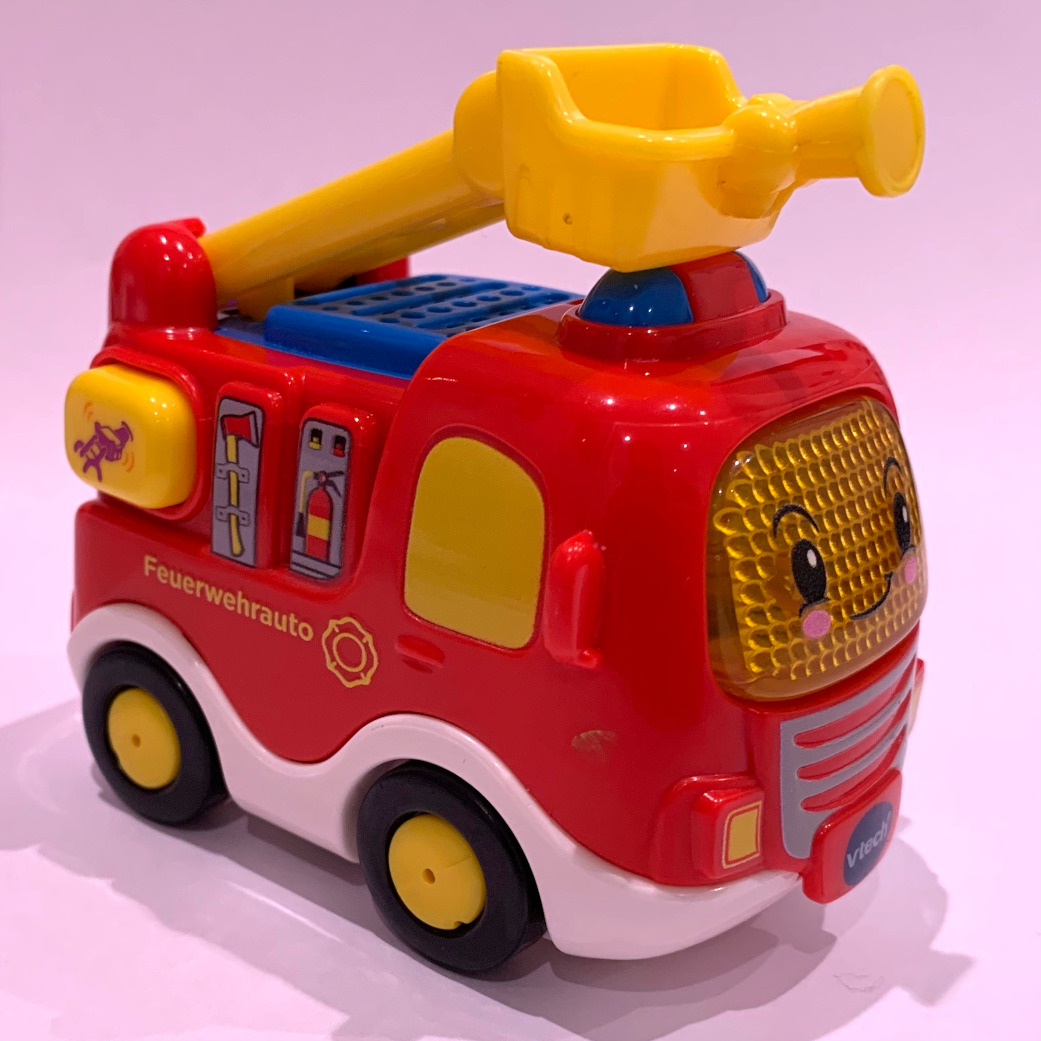
\includegraphics{img/tuttut.jpg}
	\caption{Ich bin ein Tut-Tut-Babyflitzer, ein flinkes Feuerwehrauto.}
	\label{egalWasHauptsacheEindeutig}
\end{figure}

Bilder sind wichtig. Bitte nicht versuchen die Position der Bilder selbst zu bestimmen, dass hat noch nie einen Menschen mit \LaTeX{} glücklich gemacht. Es ist aber möglich z.B. auf die Abbildung \ref{egalWasHauptsacheEindeutig} auf Seite \pageref{egalWasHauptsacheEindeutig} zu verweisen.

Genau so kann man z.B. auf Abschnitt \ref{darIchNichtVergessenUntenEinzufuegen} verweisen.


\subsection{Themenbegründung}
\label{darIchNichtVergessenUntenEinzufuegen}

Dann gibt es natürlich noch Fußnoten\footnote{Das sind diese kleinen Dinger, in denen man häufig ganz triviale Sachen erklärt.}.


\subsection{Modulbezug}
\subsection{Bezug zu den Ausbildungsstandards}
\subsection{Zielvorstellung und Leitfragen}

\subsubsection{Leitfrage 1: Wie kann ich Leitfragen schön aussehen lassen?}
\begin{tcolorbox}
So, ganz genau so ist das super, damit das niemand überliest.
\end{tcolorbox}
Hier kommt dann wieder normaler Text.

\subsubsection{Leitfrage 2: Habe ich noch etwas vergessen?}
\begin{tcolorbox}
Der Text unter Subsubsection ist natürlich nur eine verkürzte Form der Frage ob ich noch etwas vergessen habe.
\end{tcolorbox}

\subsubsection{Leitfrage 3: Auswirkung auf Lernmotivation}

\newpage
\section{Unterrichtspraxis}
\subsection{Bedingungsanalyse}
\subsubsection{Die Klassen}

Tabellen sind in \LaTeX{} evtl. auf den ersten Blick etwas unübersichtlich. Dafür gibt es aber auch sehr leicht zu bedienende Online Editoren in denen man ein wenig rumklickt und dann einfach den Code kopiert.

\begin{table}[hbtp]
\centering
\begin{tabular}{l|c|c|c|c|}
\cline{2-5}
                                & Pommes  & Cola   & Mayo    & Ketchup \\ \hline
\multicolumn{1}{|l|}{Horst}     & X       & X      & X       & X       \\ \hline
\multicolumn{1}{|l|}{Elfriede}  & X       & X      & X       &         \\ \hline
\multicolumn{1}{|l|}{Werner}    & X       & X      &         & X       \\ \hline
\multicolumn{1}{|l|}{Brösel}    & X       & X      & X       &         \\ \hline
\multicolumn{1}{|l|}{Eckhard}   & X       & X      & X       &         \\ \hline
\end{tabular}
\caption{Essensbestellung für die Pause}
\label{tab:essen}
\end{table}

\paragraph{Pommes}
Eine Auflistung der verschiedenen Ebenen mit Section, Subsection, Subsubsection, paragraph etc. findet man sehr schnell online.

\paragraph{Cola}
Nur als Beispiel.

\subsection{Planung der Unterrichtssequenzen}

\newpage
\section{Evaluation und persönliches Resümee}
\subsection{Bewertungskriterien}
\subsection{Methoden der Evaluation}
\subsection{Ergebnisse und deren Reflexion anhand von Kriterien}
Das newpage sorgt dafür, dass die Abschlussbetrachtung auf einer neuen Seite beginnt.
\newpage
\subsection{Abschlussbetrachtung}
Diese Vorlage ist mit Sicherheit nicht perfekt, aber sie wird vermutlich dem ein oder anderen das Leben etwas erleichtern.

MiKTeX (\href{https://miktex.org/}{https://miktex.org/}) ist ein empfehlenswerter \LaTeX{}-Editor für Windows.

Ich habe hier: \href{https://youtu.be/85NjaDzec8U}{https://youtu.be/85NjaDzec8U} ein Video bei YouTube hochgeladen, das kurz \LaTeX{}, das Arbeiten mit der Vorlage und den Einsatz von GitHub für die Versionsverwaltung der Hausarbeit erklärt 


% LITERATUR - HIER MUSS NIX GEÄNDERT WERRDEN!
\newpage
\thispagestyle{empty}
\bibliography{literatur}
\bibliographystyle{gerplain}

% PERSÖNLICHE ERKLÄRUNG
\newpage
\thispagestyle{empty}
\section*{Persönliche Erklärung}

Hiermit erkläre ich, dass ich die vorliegende Hausarbeit selbstständig verfasst und keine anderen als die angegebenen Hilfsmittel benutzt habe.

Die Stellen der Hausarbeit, die anderen Quellen im Wortlaut oder dem Sinn nach entnommen wurden, sind durch Angaben der Herkunft kenntlich gemacht. Dies gilt auch für Zeichnungen, Skizzen, bildliche Darstellungen sowie für Quellen aus dem Internet.

Ich bin damit einverstanden, dass diese Hausarbeit in elektronischer Form in die Bücherei des IQSH aufgenommen wird. Ich bin mir dabei bewusst, dass die Ausleihe in der Art vorgenommen wird, dass die Ausleiherin / der Ausleiher die Hausarbeit als PDF-Datei zugeschickt bekommt.

\vspace{2 cm}

\haAutorOrt, \today

\vspace{1 cm}

\parbox{5cm}{\hrule
\strut \footnotesize \haAutor}


\vfill
\section*{Anhang}
\begin{itemize}
\item Das hier ist nur eine Auflistung für das Dokument.
\item Drei Zeilen tiefer findet das Anhängen von separaten PDF Dokumenten an das generierte PDF statt.
\end{itemize}


\includepdf[pages=-]{anhang/beispiel.pdf}


\end{document}